% !TEX TS-program = xelatex

\documentclass[12pt,a4paper]{report}
\usepackage[utf8]{inputenc}
\usepackage[left=1.2in,right=1in,top=1in,bottom=1in,headheight=6pt, a4paper]{geometry} % Adjusted top margin
\usepackage{graphicx}
\usepackage{tabularx}
\usepackage{caption}
\usepackage{subcaption}
\usepackage{amsmath,amssymb,amsfonts,bbm}
\usepackage{multirow}
\usepackage{multicol}
% \usepackage[hidelinks]{hyperref}
\usepackage{cite}
\usepackage{url} 
\usepackage{enumitem}
\usepackage{svg}
\usepackage{ragged2e}
\usepackage{titlesec}
\usepackage{float}
\usepackage{placeins}
\usepackage{booktabs}
\usepackage{longtable}
\setcounter{tocdepth}{3}
\setcounter{secnumdepth}{3}
\usepackage{lipsum}
\usepackage[export]{adjustbox}
\usepackage{polyglossia}
\setdefaultlanguage{english}
\setotherlanguage{sanskrit}
\usepackage{pgfgantt}


\usepackage{fontspec}

\newfontfamily{\devanagarifont}[Script=Devanagari, Path=./]{NotoSerifDevanagari-VariableFont_wdth,wght.ttf}


%\titleformat{\subsubsubsection}[runin]{\normalfont\normalsize\bfseries}{\thesubsubsubsection}{1em}{}
%\titlespacing*{\subsubsubsection}{0pt}{3.25ex plus 1ex minus .2ex}{1.5ex plus .2ex}
%\newcommand{\subsubsubsection}[1]{\paragraph{#1}\mbox{}}
\titleformat{\chapter}[display]
    {\centering\normalfont\large\bfseries}{\MakeUppercase{\chaptertitlename} \thechapter}{2pt}{\Large}
\titlespacing{\chapter}{0pt}{0pt}{4pt}
\titleformat{\section}
  {\normalfont\large\bfseries}{\thesection}{1em}{}

\titleformat{\subsection}
  {\normalfont\normalsize\bfseries}{\thesubsection}{1em}{}

\titleformat{\subsubsection}
  {\normalfont\normalsize\bfseries}{\thesubsubsection}{1em}{}
  \renewcommand{\baselinestretch}{1.5}

\begin{document}
    \noindent
    \begin{center}
	\thispagestyle{empty}
	 \normalsize(An undertaking of Bhaktapur Municipality)\\
	 \Large\textbf{Khwopa College of Engineering}\\
	 \normalsize Affiliated to Tribhuvan University\\
	\normalsize{{{Libali-08, Bhaktapur, Nepal}}\\[0.75cm]

	\begin{figure}[h!]
		\centering
			
\includegraphics[width=0.18\textwidth]{img/khwopa logo hd.png}
	\end{figure}
	\large{A \\PROPOSAL ON\\\textbf{``Word Embedding in Nepali Language"}}\\\vspace{0.1in}
	 \normalsize{IN PARTIAL FULFILLMENT OF THE REQUIREMENT
FOR THE BACHELOR’S DEGREE IN COMPUTER ENGINEERING} \\[0.65cm]
 
\vspace*{1cm}
	
	\large\textbf{\underline{Submitted by:}}\\
	
{\bf Manish Pyakurel} (KCE077BCT020)\\
{\bf Rupak Neupane} (KCE077BCT028)\\
{\bf Sarjyant Shrestha} (KCE077BCT033)\\
{\bf Srijan Gyawali} (KCE077BCT036)\\[0.75cm]

	\large\textbf{\underline{Submitted to:}}\\

\large Department of Computer Engineering\\
\large Khwopa College of Engineering\\
\large Bhaktapur,Nepal\\[0.75cm]
\large{May, 2024}
}
\end{center}
    %\newgeometry{top=0.65in}
\pagenumbering{roman}
		%\addcontentsline{toc}{section}{Copyright}
		%\large
			%\chapter*{Copyright}
		%\normalsize
		%\justify
		%The author has agreed that the library, Khwopa College of Engineeringmay make this report freely available for inspection. Moreover, the authorhas agreed that permission for the extensive copying of this project report for scholarlypurpose may be granted by supervisor who supervised the project work recorded hereinor, in absence the Head of The Department wherein the project report was done. It isunderstood that the recognition will be given to the author of the report and toDepartment of Computer Engineering, KhCE iany use of the material of this project report. Copying or publication or other use of thisreport for financial gain without approval of the department and author’s writtenpermission is prohibited. Request for the permission to copy or to make any other useof material in this report in whole or in part should be addressed to:Head of Department\\\vspace{1.5cm}Department of Computer Engineering\\Khwopa College of Engineering(KhCE)\\Liwali,\\Bhaktapur, Nepal.\\\break

	
	   % \addcontentsline{toc}{section}{Acknowledgement}
		%\large
			%\chapter*{Acknowledgement}
		%\normalsize
		% We would like to thank \textbf{Er. Anish Baral} for his wise counsel, inspiring ideas, and invaluable direction, help, and support throughout this project. We also owe a debt of gratitude to \textbf{Er. Dinesh Gothe} and \textbf{Er. Mukesh Kumar Pokharel} \textbf for their tireless efforts at every stage of the project, as well as for their insightful counsel and recommendations.\\ We are truly grateful for the wisdom and support they have provided us and it isthrough their efforts that we have been able to bring this project to fruition. Onbehalf of the entire team, we express our sincere thanks and appreciation for their invaluable contributions.\\
            


        %\begin{tabular}{p{1.5in}p{3in}}
			%Bijay Kadariya & KCE076BCT013\\
			%Prajwal Acharya & KCE076BCT025\\
			%Prajwal Shrestha & KCE076BCT026\\
			%Sameer Shrestha & KCE076BCT037\\
		%\end{tabular}
		%\break
		
		
		\addcontentsline{toc}{section}{Abstract}
		\large
			\chapter*{Abstract}
		\normalsize
        \noindent
		In recent years, Natural Language Processing (NLP) has made significant strides, particularly in the development of word embeddings that capture both semantic and syntactic meanings of words. This proposal focuses on creating word embeddings for the Nepali language, which remains underrepresented in the realm of NLP due to its complex grammatical structure and rich character set. Despite the progress in NLP, low-resource languages like Nepali face challenges in data collection and model training. This study aims to address these challenges by leveraging pre-trained models and fine-tuning them with a substantial Nepali corpus. The proposed system will utilize transformer-based models, such as BERT, to generate contextualized word embeddings that can be applied to various NLP tasks, including sentiment analysis, machine translation, and question answering. By advancing NLP technologies for the Nepali language, we aim to enhance digital accessibility and empower communities through improved communication and educational tools.

		\noindent
		\textbf{Keywords}: 
		\textit{Word Embeddings, Nepali Language, Natural Language Processing, BERT, Transformer Models, Contextualized Embeddings, Low-Resource Languages.\\
 }\\

		\break


	    \tableofcontents

		% \addcontentsline{toc}{section}{List of Tables}
		% \listoftables
		\break
		\pagebreak

		\addcontentsline{toc}{section}{List of Figures}
		\listoffigures
		\break
	
	
	
		\addcontentsline{toc}{section}{List of Symbols and Abbreviation}
		\Large
			\begingroup
				\let\clearpage\relax
				\chapter*{List of Symbols and Abbreviation}
			\endgroup
   
		\normalsize
		\begin{tabular}{p{1in}p{5in}} 
			AI & Aritificial Intelligence\\
			BERT & Bidirectional Encoder Representations from Transformers\\
			% BLEU & Bilingual Evaluation Understudy\\
			% CNN & Convolutional Neural Network\\
			% GAN & Generative Adversarial Network\\
			% GPU & Graphics Processing Unit\\
			% LDA & Latent Dirichlet Allocation\\
			% LSTM & Long Short-Term Memory\\
			% ML & Machine Learning\\
			% MSE & Mean Squared Error\\
			% NER & Named Entity Recognition\\
			NLP & Natural Language Processing\\
			NLTK & Natural Language Toolkit\\
			% PCA & Principal Component Analysis\\
			% POS & Part-of-Speech\\
			% RNN & Recurrent Neural Network\\
			% RMSE & Root Mean Squared Error\\
			% ROC & Receiver Operating Characteristic\\
			% SGD & Stochastic Gradient Descent\\
			% SOTA & State-of-the-Art\\
			% SVM & Support Vector Machine\\
			TF-IDF & Term Frequency-Inverse Document Frequency\\
			XLM & Cross Lingual Language Model\\
			% WER & Word Error Rate\\
			\end{tabular}





		\break
		\pagebreak
		
	
    \chapter{Introduction}
\pagenumbering{arabic}
\section{Background Introduction}
NLP is a branch of linguitics, computer science, and artificial intelligence concerned with computer human interaction, mainly how to design computers to process and evaluate huge volumes of natural language data \cite{asudani2023impact}. Pre-training of an NLP model plays an essential role in transfer learning, where a language model will be trained on a vast corpus set and later fine-tune the model for a specific purpose \cite{NepaliBERT}. Word embedding is a fundamental concept in NLP. It is a real-valued vector representation of words by embedding both semantic and syntactic meanings obtained from unlabeled large corpus \cite{Wang_Wang_Chen_Wang_Kuo_2019}. It is of n-dimensional distributed representation of a text that attempts to capture the meanings of the words \cite{asudani2023impact}. Word embeddings can be obtained using language modeling and feature learning techniques, where words or phrases from the vocabulary are mapped to vectors of real numbers \cite{enwiki:1219561882}. Pre-trained word embeddings encode general word semantics and lexical regularities of natural language, and have proven useful across many NLP tasks, including word sense disambiguation, machine translation, and sentiment analysis, to name a few \cite{moreo2019wordclass}. Word embeddings have been found to be very useful for many NLP tasks, including but not limited to Chunking \cite{turian-etal-2010-word}, Question Answering \cite{questionanswer}, Parsing and Sentiment Analysis\cite{sentimentanalysis}. \cite{wordembedding} \\\\
\textbf{Types of Word Embedding Techniques} \cite{reviewOnWordEmbedding} \\
\textbf{Traditional Embeddings}: Traditional word embeddings represent words as fixed vectors in an n-dimensional space, capturing semantic relationships between words.
These embeddings are static and do not change based on context or training data. \\
\textbf{Static Embeddings}:
Static word embeddings are pre-trained on a large corpus of text and do not change during model training.
They are useful for tasks where word meanings remain constant across different contexts.\\
\textbf{Contextualized Embeddings}:
Contextualized word embeddings, like BERT, are based on transformer models that can capture word meanings based on the context in which they appear.
These embeddings provide more accurate representations of words by considering the surrounding context during training. \\
\textbf{Combined Word Embedding and Neural Network Models}:
Combining word embeddings with neural network models can enhance model accuracy in various natural language processing tasks such as sentiment classification, text categorization, and phrase prediction. \\
Nepali is one of the languages that uses Devanagari, a script used in many languages spoken in Asian countries. It is spoken by more than 20 million people, mainly in Nepal, and other places in the world including Bhutan, India and Myanmar \cite{niraula2020linguistic}.  It has been rarely used for Natural Language Processing services.  Nepali can be quite complex due to its many sounds, grammar rules, and ways to change words. Due to its complex grammatical structure and rich characters, extracting fruitful information from the corpus has been challenging \cite{NepaliBERT}.\\
The advancement of NLP technologies adapted to individual languages, like Nepali, hold immense potential for empowering communities and enhancing accessibility to digital resources for Nepali language. By filling the gap between technological innovation and linguistic diversity, we can unlock new possibilities for communication and education.\\
\section{Problem Statement} 
Even though Word Embeddings can be directly learned from raw texts in an unsupervised fashion, gathering a large amount of data for its training remains a huge challenge in itself for a low-resource language such as Nepali \cite{koirala-niraula-2021-npvec1}. Despite having breakthroughs in the field of NLP, productive results with the Nepali language have not been achieved. One of the primary reasons for this is the need for more computational resources \cite{NepaliBERT}. As mentioned in the most recent study in this topic (i.e NepaliBERT \cite{NepaliBERT}), there is a lack of larger, more diverse, and context-rich dataset to enhance the accuracy and robustness of the word embeddings in Nepali language. This research study seeks to construct a more finely tuned model capable of generating embeddings for the Nepali corpus. It is seen that there is reduction of perplexity by using XLM.
\section{Objective}
    The main aim of this project is:
    \begin{itemize}
        \item To develop context dependent word embedding for Nepali language.
    \end{itemize}

    \chapter{Literature Review}
\noindent
Most of the research that has been undertaken on the Nepali corpus was focusing on generating embeddings through traditional approaches like TFIDF, Wod2Vec and other embedding methods. \cite{Bhatta_Shrestha_Nepal_Pandey_Koirala_2020} \cite{Singh2019NepaliMT} \cite{shahi2018nepali} and \cite{ghosh2018class} implemented TF-IDF on Nepali text for text classification and other purposes such as sentiment analysis. Similarly, Word2Vec approach in nepali corpus was implemented by \cite{Bhatta_Shrestha_Nepal_Pandey_Koirala_2020} \cite{kaushal2016} and \cite{basnet2018improving}. 300-Dimensional Word Embeddings for Nepali Language \cite{300D} has pre-trained Word2Vec model having 300-dimensional vectors for more than 0.5 million Nepali words and phrases. The embeddings generated using the methods described above are static, implying that each word retains only one vector representation regardless of its context of use. However, contemporary trends emphasize the adoption of contextual-dependent embeddings over their contextual-independent counterparts. As highlighted earlier, there have been limited studies on BERT within the Nepali context. \cite{koirala-niraula-2021-npvec1} claimed to provide an efficient Nepali BERT embedding, but despite having a huge dataset they were short of computational resources due to which they had to compromise on the different BERT parameters. They modified the BERT model by averaging the hidden states from the last two hidden layers to get the embeddings, whereas, for getting the baseline results, instead of using any pre-trained word vectors, a trainable Keras embedding layer was used in front of the architecture mentioned above which automatically learns the word embeddings by only using the provided training examples. \cite{rajan_nepalibert_2021} and  \cite{milanmg_bert-nepali_2022} also tried the capacity of BERT for cross-lingual in Natural Language Processing. \\\\
There are also studies done in XLM \cite{NEURIPS2019_c04c19c2}. The paper compares a Nepali language model with a cross-lingual language model trained in Nepali but enriched with different combinations of Hindi and English data, showing how leveraging data from related languages can benefit low-resource languages like Nepali.
300-Dimensional Word Embeddings for Nepali Language \cite{300D} has pre-trained Word2Vec model having 300-dimensional vectors for more than 0.5 million Nepali words and phrases.
The embeddings generated using the methods described above are static, implying that each word retains only one vector representation regardless of its context of use. However, contemporary trends emphasize the adoption of contextual-dependent embeddings over their contextual-independent counterparts. As highlighted earlier, there have been limited studies on BERT within the Nepali context. \cite{koirala-niraula-2021-npvec1} claimed to provide an efficient Nepali BERT embedding, but despite having a huge dataset they were short of computational resources due to which they had to compromise on the different BERT parameters. They modified the BERT model by averaging the hidden states from the last two hidden layers to get the embeddings, whereas, for getting the baseline results, instead of using any pre-trained word vectors, a trainable Keras embedding layer was used in front of the architecture mentioned above which automatically learns the word embeddings by only using the provided training examples. \cite{rajan_nepalibert_2021} and  \cite{milanmg_bert-nepali_2022} also tried the capacity of BERT for cross-lingual in Natural Language Processing. \\\\
There are also studies done in XLM \cite{NEURIPS2019_c04c19c2}. The paper compares a Nepali language model with a cross-lingual language model trained in Nepali but enriched with different combinations of Hindi and English data, showing how leveraging data from related languages can benefit low-resource languages like Nepali.

    \chapter{Theoretical Background}
\section{Transformers}
        A transformer model is a neural network that learns context and thus meaning by tracking relationships in sequential data like the words in this sentence.
        Transformer models apply an evolving set of mathematical techniques, called attention or self-attention, to detect subtle ways even distant data elements in a series influence and depend on each other.
        First described in a 2017 paper from Google\cite{vaswani2023attention}, transformers are among the newest and one of the most powerful classes of models invented to date. They’re driving a wave of advances in machine learning some have dubbed transformer AI.
        Stanford researchers called transformers “foundation models” in an August 2021 paper\cite{bommasani2021opportunities} because they see them driving a paradigm shift in AI.

        \begin{figure}[hbt!]
            \center{
                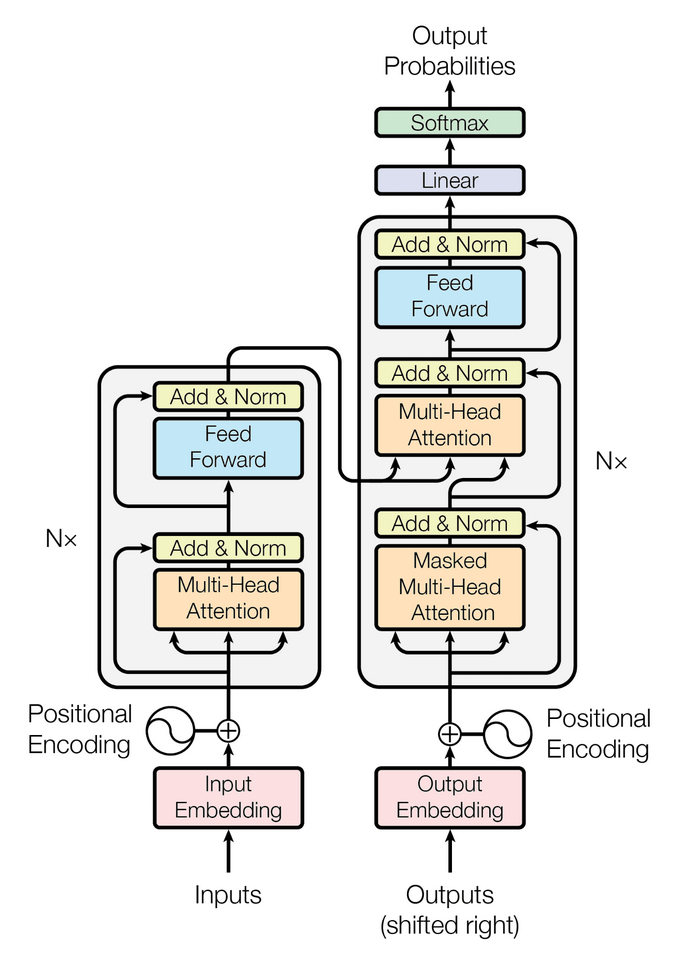
\includegraphics[width=0.46\textwidth]{./img/attention_research_1.png}
                \caption{The Transformer - model architecture.\cite{vaswani2023attention}}
                }
        \end{figure}

\section{BERT}
    BERT stands for Bidirectional Encoder Representations from Transformers. It is designed to train deep bidirectional representations from unlabeled text by jointly conditioning on both left and right context \cite{devlin2019bert}. BERT utilizes the Transformer architecture, which employs an attention mechanism to understand contextual relationships among words or sub-words within a text. The basic Transformer structure consists of two distinct components: an encoder, which processes the input text, and a decoder, which generates predictions for the given task. BERT architecture enables it to handle various NLP tasks effectively, such as question answering, sentiment analysis, and text classification, by fine-tuning on specific datasets. 

    \begin{figure}[hbt!]
        \center{
            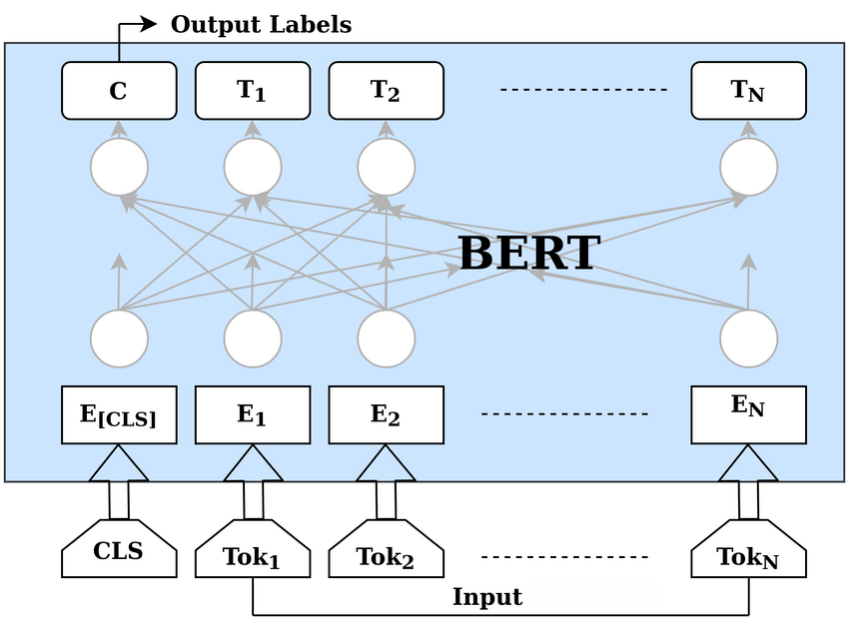
\includegraphics[width=1\textwidth]{./img/bertarchitecture.png}
            \caption{Illustrations of Fine-tuning BERT on Different Tasks.\cite{Gundapu}}
            }
    \end{figure}

    \chapter{Methodology}
\section{Software Development Approach}
Agile development is a software development approach that emphasizes incremental progress and rapid cycles. It involves releasing small increments of functionality that build upon previous versions. Thorough testing is conducted for each release to ensure software quality. Agile is often employed for time-critical applications. Although this project is not time-critical this model seems to be the most optimal and practical in our case.
\begin{figure}[hbt!]
    \center{
        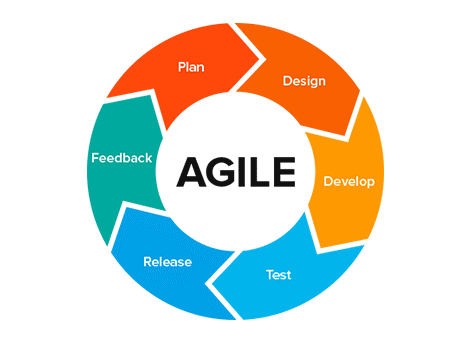
\includegraphics[width=0.75\textwidth]{./img/agile.png}
        \caption{Agile Model for Software Development}
        \subcaption*{\textit{source: \textcolor{blue}{https://mobilelive.medium.com/agile-development-a-comprehensive-guide-for-the-modern-era-d2fe9ae7b395}}}
    }
\end{figure}
\newpage
\section{Proposed System Block Diagram}
    \begin{figure}[hbt!]
    \center{
        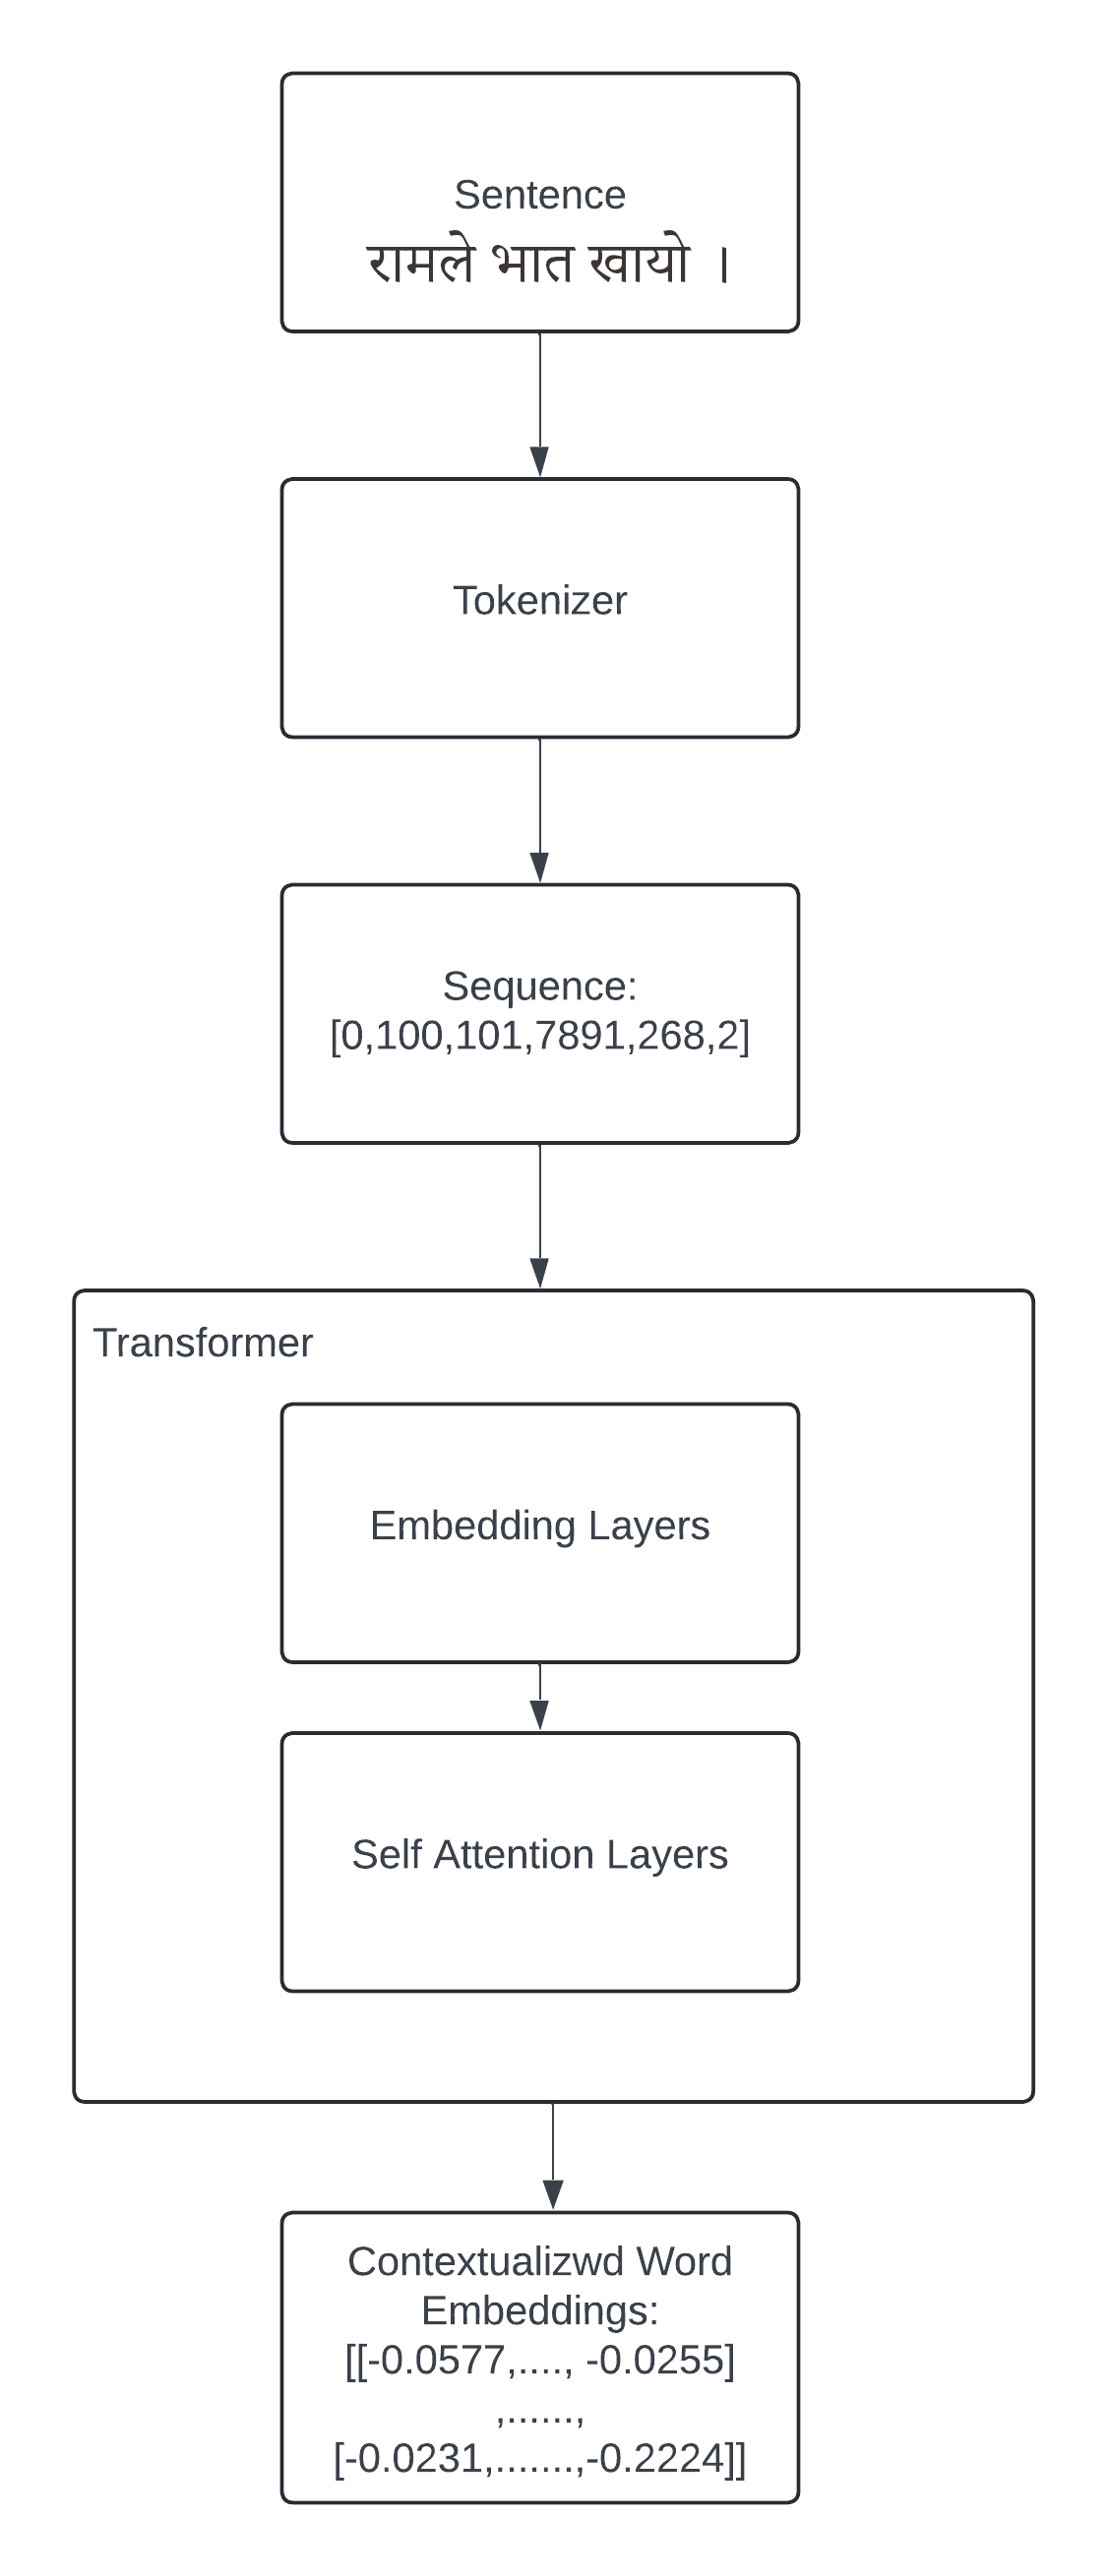
\includegraphics[width=0.6\textwidth]{./img/Block_Diagram.png}
        \caption{Block diagram of Proposed Sytem}
        }
    \end{figure}

\section{Description of Working Flow of Proposed System}
\begin{enumerate}
    \item \textbf{Sentence Input}:
    \begin{itemize}
        \item The process starts with a given sentence in the Nepali language: \textsanskrit{रामले भात खायो}
    \end{itemize}
    
    \item \textbf{Tokenizer}:
    \begin{itemize}
        \item The sentence is passed to a tokenizer, which breaks down the sentence into individual tokens. The tokens are then converted into a sequence of numerical IDs. For example, the sentence \textsanskrit{रामले भात खायो} is converted into the sequence \texttt{[0, 100, 101, 7891, 268, 2]}.
    \end{itemize}
    
    \item \textbf{Transformer Model}:
    \begin{itemize}
        \item The tokenized sequence is then fed into a Transformer model, which consists of several layers. This model processes the sequence to generate contextualized word embeddings.
        
        \begin{itemize}
            \item \textbf{Embedding Layers}:
            \begin{itemize}
                \item The first part of the Transformer model is the embedding layers. These layers convert the input token IDs into dense vectors of fixed size. These vectors capture semantic information about the words.
            \end{itemize}
            
            \item \textbf{Self-Attention Layers}:
            \begin{itemize}
                \item After the embedding layers, the vectors pass through multiple self-attention layers. These layers allow the model to weigh the importance of different words in the sentence relative to each other, thereby capturing the context of each word in relation to the entire sentence.
            \end{itemize}
        \end{itemize}
    \end{itemize}
    
    \item \textbf{Contextualized Word Embeddings Output}:
    \begin{itemize}
        \item The final output of the Transformer model is a set of contextualized word embeddings. Each word in the input sentence is now represented by a vector that encodes both its meaning and its context within the sentence. For example, the embeddings might look like:
        [[-0.0577, ..., -0.0255],
         ...,
         [-0.0231, ..., -0.2224]].
    \end{itemize}
\end{enumerate}

% \section{Performance Evaluation Metrics}

    \chapter{System Design}
\section{Requirement Analysis}
        \subsection{Functional Requirements}
            These are specifications that describe the fundamental capabilities and behaviors a system or product must exhibit to meet the users' needs and achieve its intended purpose. 

            \subsubsection{Tokenization}
            The system should be able to tokenize Nepali text into individual words or subword units, considering the complexities of the Nepali script.

            \subsubsection{Embedding Generation}
            Generate dense vector representations (embeddings) for each word or subword unit in the Nepali vocabulary. These embeddings should capture semantic relationships between words.

            \subsubsection{Embedding Lookup}
            Allow users to retrieve the embedding vector for any given word or subword unit in the Nepali vocabulary.

            \subsubsection{Similarity Calculation}
            Calculate semantic similarity between words or subword units based on their embedding vectors. Users should be able to compare words and get similarity scores.

        \subsection{Non-Functional Requirements}
            These are the characteristics and qualities that describe how a system should behave and perform.

            \subsubsection{Usability}            
            The system should have a user-friendly interface or API that allows users to easily interact with word embeddings without requiring deep technical knowledge.

            \subsubsection{Reliability}
            The system aims to be highly available, with minimal downtime, to ensure users can access word embedding functionalities when needed.

            \subsubsection{Interoperability}
            The system ensures compatibility with various operating systems, programming languages, and NLP frameworks to facilitate integration with existing systems and workflows.

            \subsubsection{Maintainability}            
            The system with a modular architecture will enable easy maintenance, updates, and future enhancements.


        % \newpage        
        \subsection{Feasibility Study}
            The following points describes the feasibility of the project.

            \subsubsection{Economic Feasibility}
                The total expenditure of the project is just computational power. The computational resources can be fulfilled with the help of college. Therefore, the project is economically feasible.

            \subsubsection{Technical Feasibility}
                While existing datasets on this topic are available, they are insufficient. But, by using the abundance of Nepali news articles, books, and literature accessible online can augment our corpus significantly through web scraping.

            \subsubsection{Operational Feasibility}
                The operational processes, including web-scraping and model training, are well-defined and can be efficiently carried out by the project team. Additionally, the project aligns with the existing technical infrastructure and capabilities, making it operationally feasible.
%\textbf{Note: All the diagram is not mandatory..select according to the type of project you are going to do.}
    \chapter{Implementation Plan}
\section{Schedule(Gantt Chart)}
\vspace{2em}
        \begin{figure}[htbp]
            \hspace*{-1cm} % Adjust the value as needed
            \begin{ganttchart}[
                hgrid,
                vgrid,
                x unit=2.5em,
                y unit chart=4em,
                time slot format=isodate-yearmonth,
                time slot unit=month,
                title height=1,
                bar/.append style={fill=blue!40},
                bar height=0.7,
                bar label node/.append style={align=right, text width=7em},
                group height=0.6,
                group peaks height=0.2,
                group peaks tip position=0,
                group/.append style={draw=black, fill=green!50},
                group label font=\small
                ]{2024-04}{2025-03}
                \gantttitlecalendar{year} \\
                \gantttitlecalendar{month} \\
                \ganttbar{Requirement Analysis}{2024-04}{2024-05} \\
                \ganttbar{Feasibility Study}{2024-04}{2024-05} \\
                \ganttbar{Software Design}{2024-05}{2024-06} \\
                \ganttbar{Implementation}{2024-06}{2025-01} \\
                \ganttbar{Testing}{2025-01}{2025-02} \\
                \ganttbar{Research}{2024-04}{2025-01}\\
                \ganttbar{Documentation}{2024-04}{2025-03}\\
            \end{ganttchart}
            \caption{Gantt Chart}
        \end{figure}
\newpage
\section{Hardware and Software requirements}
    \subsection{Software Requirement}
    This project requires following softwares:
    \subsubsection*{Python} 
    Python is our primary language for this project, chosen for its versatility and simplicity. All machine learning frameworks are imported using Python, leveraging its dominant position in data science and machine learning. This allows us to seamlessly integrate powerful libraries like TensorFlow and PyTorch for efficient model development. It also provides essential libraries like Scikit-learn, Numpy, Pandas, etc.

    \subsubsection*{Pytorch}
    Pytorch is a an open-source machine learning framework. It provides a flexible and dynamic computational graph, which allows for easy experimentation and rapid development of deep learning models. 

    \subsubsection*{Natural Language Toolkit}
    Natural Language Toolkit (NLTK) is a free and open source Python library for natural language processing. NLTK provides stemming, lowercase, categorization, tokenization, spell check, lemmatization, and semantic reasoning text processing packages. It gives access to lexical resources like WordNet.


    \subsection{Hardware Requirement}
    \subsubsection*{Memory}
    Word embedding models like BERT need a lot of memory to work. Training BERT needs several gigabytes of RAM, maybe even more if the model is really big. 

    \subsubsection*{Processing Power}
    Training these models takes a lot of computing power, especially when working with big datasets or complex models. Having a strong computer with a good CPU or GPU can help speed up the training process. GPUs are especially useful for this because it can handle lots of tasks at once.

    \subsubsection*{Storage Space}
    Storing all the data and models can take up a lot of space. Adequate disk space is required to store necessary files, including the dataset, the models, and any other files related to the project.

% \section{Cost Estimation}


    \chapter{Work Completed}
\section{Dataset Preparation}
\begin{itemize}
    \item \textbf{Data Loading:} The project uses the \textit{Kantipur} dataset, which consists of Nepali news articles. This data is loaded from a cleaned and combined TSV file. The data is organized into two columns: one for the \textit{title} of the article and another for the \textit{news content}.
    \item \textbf{Text Processing:} The raw Nepali text from the dataset is processed for tokenization. The custom tokenizer ensures that the text is cleaned and normalized, addressing issues like extra spaces and Unicode variations in Nepali characters.
\end{itemize}

\section{Tokenizer Development}
\begin{itemize}
    \item \textbf{NepaliTokenizer:} A specialized tokenizer was implemented for Nepali text, called \texttt{NepaliTokenizer}. This class was designed to handle the unique features of the Nepali language, including:
    \begin{itemize}
        \item \textit{Character Ranges:} It checks whether a character falls within the Devanagari script (the script used for Nepali) and processes it accordingly.
        \item \textit{Punctuation Handling:} It accounts for Nepali punctuation marks (\textsanskrit{।}, \textsanskrit{॥}, and others) and ensures they are treated as distinct tokens during tokenization.
        \item \textit{Suffix Handling:} Common Nepali suffixes and postpositions (like \textsanskrit{ले}, \textsanskrit{को}, \textsanskrit{बाट}) are identified and separated as individual tokens to preserve their semantic roles in the language.
    \end{itemize}
    \item \textbf{CustomBERTTokenizer:} A more advanced tokenizer, \texttt{CustomBERTTokenizer}, was built to handle:
    \begin{itemize}
        \item \textit{Vocabulary Building:} This tokenizer automatically builds a vocabulary of frequent words and tokens based on the input dataset. It dynamically updates the vocabulary while ensuring it does not exceed the predefined maximum size (30,000 tokens).
        \item \textit{Token Masking:} During pretraining, certain tokens are randomly masked (\texttt{[MASK]}) to create a Masked Language Modeling (MLM) task, which is a core part of training BERT models.
        \item \textit{Encoding:} The tokenizer converts raw text into token IDs, adding special tokens such as \texttt{[CLS]} (for classification), \texttt{[SEP]} (to separate segments), and \texttt{[PAD]} (for padding sequences to a uniform length).
    \end{itemize}
\end{itemize}

\section{Dataset Processing}
\begin{itemize}
    \item \textbf{Data Preparation for Pretraining:} The dataset is prepared specifically for BERT pretraining, where the model learns to predict masked tokens (a form of unsupervised learning). For each article in the dataset:
    \begin{itemize}
        \item \textit{Input Sequences:} The raw text is encoded into a sequence of token IDs.
        \item \textit{Segment IDs:} Segment IDs are created, marking which tokens belong to which segment.
        \item \textit{Masked Tokens:} For the MLM task, some tokens in the sequence are randomly masked, and the model is trained to predict these missing words. The masked tokens are tracked for loss calculation during training.
    \end{itemize}
\end{itemize}

\section{Model Architecture}
\begin{itemize}
    \item \textbf{BERT Embedding Layer:} A custom embedding layer was built that includes:
    \begin{itemize}
        \item \textit{Token Embeddings:} Maps each token in the vocabulary to a dense vector.
        \item \textit{Segment Embeddings:} Differentiates between multiple segments (useful for tasks like question answering).
        \item \textit{Positional Embeddings:} Positional embeddings are added to provide information about the order of tokens in the sequence.
        \item \textit{Dropout:} A dropout layer is included to prevent overfitting during training.
    \end{itemize}
    \item \textbf{Transformer Encoder:} The core of the BERT model is the Transformer Encoder, which processes sequences of token embeddings using attention mechanisms to capture relationships between tokens at various positions in the input sequence.
    \item \textbf{Pretraining Head (MLM):} The MLM head predicts the original tokens that were masked during pretraining. This is achieved by using a linear layer over the final hidden states produced by the encoder.
\end{itemize}

\section{Training Loop}
\begin{itemize}
    \item \textbf{Training Workflow:} The model is trained using a cross-entropy loss function, which measures how well the predicted token IDs match the original token IDs. The optimizer (Adam) updates the model parameters to minimize this loss. The training loop runs over multiple epochs.
    \item \textbf{Validation Workflow:} The model's performance is evaluated on the validation set after each epoch. The validation loss is calculated using the same MLM loss function.
    \item \textbf{Loss Tracking:} Loss values for both the training and testing datasets are recorded after each epoch, and these are saved into text files for further analysis.
\end{itemize}

\section{Data Splitting and Loader Implementation}
\begin{itemize}
    \item \textbf{Training and Validation Split:} The dataset is divided into training and validation sets, with 80\% used for training and 20\% for validation.
    \item \textbf{DataLoader Implementation:} DataLoaders are used to manage batching, shuffling, and pinning memory for efficient data loading during training and testing.
\end{itemize}

\section{Performance Metrics}
Loss during training and validation is recorded and plotted against epochs to monitor performance improvements. A plot showing the loss values over epochs is generated, allowing us to monitor the model's training progress.
\begin{figure}[hbt!]
    \center{
        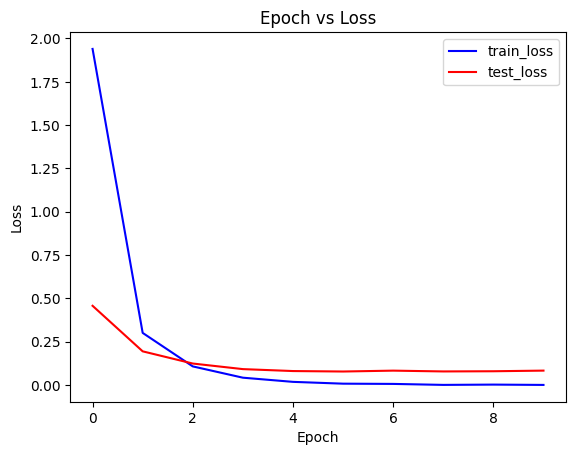
\includegraphics[width=1\textwidth]{./img/training-graph.png}
        \caption{Training graph}
    }
\end{figure}

\section{Future Work}

Our ongoing efforts focus on generating and evaluating Nepali text embeddings for enhanced information retrieval and related applications. The following steps outline the key areas of work in progress:

\begin{enumerate}
    \item \textbf{Embedding Generation:}
    \begin{itemize}
        \item Generate embeddings using the \textit{original model} and the \textit{fine-tuned model} on test articles to avoid data leakage from training data.
    \end{itemize}

    \item \textbf{Text Splitting:}
    \begin{itemize}
        \item Apply techniques such as \textit{LangChain recursive splitting} to divide articles into smaller text chunks, facilitating effective embedding and retrieval.
    \end{itemize}

    \item \textbf{Embedding Comparison:}
    \begin{itemize}
        \item Compare embeddings from both models for each text chunk using similarity metrics such as \textit{cosine similarity} or other distance measures.
    \end{itemize}

    \item \textbf{Question Generation:}
    \begin{itemize}
        \item Use high-performing language models, such as \textit{LLaMA 3.1 70B}, to generate contextually relevant questions from the text chunks.
    \end{itemize}

    \item \textbf{Information Retrieval Evaluation:}
    \begin{itemize}
        \item Retrieve \textit{Top-K text chunks} based on embedding similarity scores for each question and evaluate performance using metrics like \textit{hit rate}.
    \end{itemize}

    \item \textbf{LLM Response Testing:}
    \begin{itemize}
        \item Validate the retrieved information by prompting the LLM with retrieved text and assessing its accuracy in answering the generated questions.
    \end{itemize}

    % \item \textbf{Advanced Retrieval Optimization:}
    % \begin{itemize}
    %     \item Experiment with \textit{graph-based embedding storage} for improved retrieval accuracy and efficiency.
    % \end{itemize}

    % \item \textbf{Future Scope:}
    % \begin{itemize}
    %     \item Extend embeddings to other applications, such as \textit{sentiment analysis} and \textit{recommendation systems}.
    %     \item Optimize information retrieval for \textit{low-resource languages} and evaluate performance using tools such as \textit{RAGAS}.
    % \end{itemize}
\end{enumerate}

This approach provides a structured framework for evaluating the fine-tuned model while enabling future advancements in information retrieval and related applications.


    \chapter{Work to be done}
\section{Expand Dataset Further}
Increase the size and diversity of the dataset by collecting more Nepali legal texts. This will improve the model's ability to generalize and perform well on a wider range of inputs.

\section{Prepare Transformer-Based Embedding Layer and Self-Attention Layers}
Implement the core components of a transformer model, including embedding layers to convert words into numerical representations and self-attention layers to capture dependencies between words in the text. These components are crucial for understanding contextual relationships within the data.

\section{Train, Test, and Validate the Model}
Train the model using the expanded dataset to learn from the data and optimize its performance on legal text tasks. Test the model on separate datasets to evaluate its accuracy and generalization capabilities. Validate the model's performance against predefined metrics to ensure it meets quality standards.

\section{Hyperparameter Tuning}
Fine-tune the model by adjusting hyperparameters such as learning rate, batch size, and dropout rates. This process aims to optimize model performance and efficiency, leading to better results during training and inference.
   
    %\printbibliography[title={References}] % Print bibliography with the title "References"
    %\bibliographystyle{IEEEtran}
    %\bibliography{ref}
    %\addcontentsline{toc}{section}{Bibliography}
    \newpage
      % \renewcommand{\bibname}{References}
      \bibliographystyle{unsrt}
       \bibliography{ref}
       \addcontentsline{toc}{chapter}{References}
\end{document}
